\chapter{Zusammenfassung}

In diesem Kapitel wird ein Rückblick auf die Arbeit gegeben und die Ergebnisse zusammengefasst.
Zudem werden die Ergebnisse bewertet indem ein Fazit über die Effektivität und Usability der entwickelten Konzepte gezogen wird.
Dabei wird auch auf die Herausforderungen und Schwierigkeiten eingegangen, die bei der Umsetzung der Konzepte aufgetreten sind.
Zuletzt wird ein Ausblick auf mögliche Weiterentwicklungen der Konzepte gegeben.

\section{Ergebnisse}

Im Rahmen der Bachelorarbeit wurden zwei Interaktionskonzepte für die Visualisierung von Requirements in Augmented Reality ausgearbeitet und in einem Prototypen umgesetzt.
Der Prototyp ist dabei eine WebXR-Anwendung, die mit dem Framework Babylon.js in TypeScript entwickelt wurde.
Die Anwendung kann direkt von einem AR-fähigen Browser aufgerufen werden und ist somit plattformunabhängig.



Das erste Konzept ist die Visualisierung von Requirements in Kombination mit einem möglichst akkuraten 3D-Modell des zu entwickelnden Produkts.
Dabei wird das 3D-Modell vom Nutzer auf einer freien Fläche im Raum platziert und kann in einer \glqq{}Explosions\grqq{}-Animation, welche in Abbildung \ref{fig:porsche-explosion-ar} anhand einer Bildsequenz dargestellt ist, in seine Bauteile zerlegt werden.
Ist das Modell in seine Einzelteile zerlegt, werden die Anforderungen als Panels an den einzelnen Bauteilen visualisiert.
Der Nutzer kann dann die Animation wieder rückwärts abspielen, um das Modell wieder zusammenzusetzen.
Dabei verschwinden die Anforderungen wieder, und das Produkt kann in seinem originalen Gesamtzustand ohne Requirements betrachtet werden.
Im Prototyp wurde dafür ein Auto-Modell verwendet, welches in einer Animation des ganzen Autos in seine Einzelteile zerlegt wird.
Zur Visualisierung der eingeplanten Detailansicht können im Prototyp außerdem die Räder des Modells angeklickt werden, um so eine Detailansicht der Anforderungen an die Räder zu erhalten.
Das Interaktionskonzept zeigt dabei viel Potenzial, um viele Interaktionsmöglichkeiten mit dem 3D-Modell und den Anforderungen zu ermöglichen.
Ein großer Mehrwert der Visualisierung in AR ist dabei, dass das 3D-Modell in Originalgröße dargestellt werden kann und so eine realistische Darstellung des Produkts ermöglicht wird.

\begin{figure}[H]
    \centering
    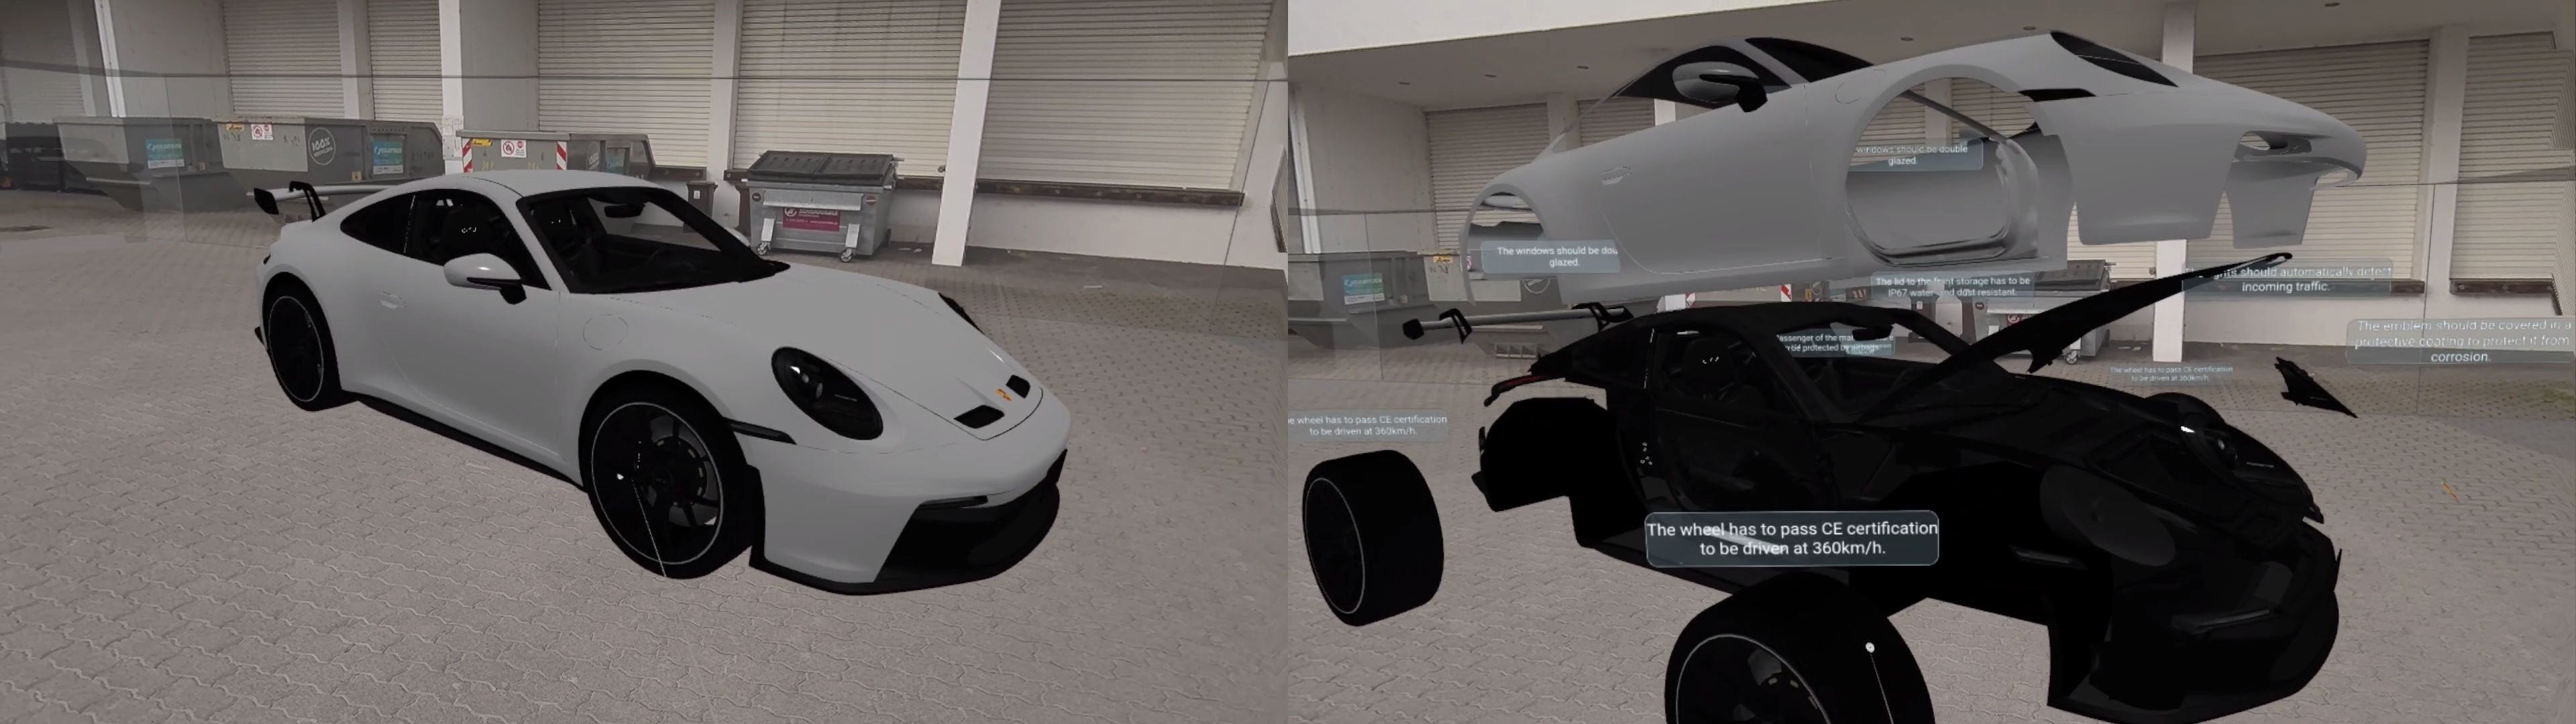
\includegraphics[width=1\textwidth]{images/PorscheExplosionAR.png}
    \caption{Bildsequenz aus dem Prototyp der Explodierenden Bauteile in AR}
    \label{fig:porsche-explosion-ar}
\end{figure}

Das zweite Konzept ist die Visualisierung von Requirements in Wolken aus Textpanels, die in der AR-Umgebung schweben.
Die Wolken sind dabei Cluster von Anforderungen, die thematisch zusammengehören.
Zusätzlich können die Anforderungen in den Wolken angeklickt werden, um zugehörige Anforderungen anzuzeigen.
Dieses Konzept ist deutlich einfacher automatisiert umzusetzen, da die Anforderungen in den Wolken nur als Textpanels dargestellt werden und keine extra Animationen oder 3D-Modelle benötigt werden.

Jedoch ist auch der Mehrwert für den Nutzer in diesem Konzept geringer, da es weniger Möglichkeiten zur Interaktion in Augmented Reality gibt als im ersten Konzept.
Zudem treten bei der dreidimensionalen Darstellung der Anforderungswolken Herausforderungen auf, die in einer 2D-Darstellung nicht auftreten würden.
Beispielsweise werden oft Anforderungen hintereinander angezeigt, sodass der Nutzer die Anforderungen nur schwer oder gar nicht mehr lesen kann.
Auch können nicht sehr viele Anforderungen in einer Wolke dargestellt werden, da die Anforderungen sonst zu klein werden und nicht mehr lesbar sind.
Aufgrund der wenigen AR spezifischen Interaktionsmöglichkeiten und der Probleme der Darstellung des Konzepts im dreidimensionalen Raum ist fraglich, ob das Konzept in AR einen Mehrwert gegenüber einer 2D-Darstellung eines ähnlichen Konzepts bietet.



\section{Fazit}

Insgesamt konnte in dieser Arbeit gezeigt werden, dass die Visualisierung von Requirements in Augmented Reality zumindest in einem Prototypen umsetzbar ist.
Das erste Konzept zeigt dabei auch, dass mit der Visualisierung in AR durch viele neue Interaktionsmöglichkeiten ein Mehrwert in der Visualisierung von Requirements erreicht werden kann.

In AR können, wie vor allem am Konzept der explodierten 3D-Modelle gezeigt wurde, viele neue Interaktionsmöglichkeiten geschaffen werden, die in einer 2D-Darstellung nicht möglich wären.
Physische Produkte und ihre Bauteile können in Originalgröße dargestellt und interaktiv mit ihren Anforderungen verknüpft werden.
So entsteht ein neuer Ansatz, um Anforderungen besser zu verstehen, zu kommunizieren und zu visualisieren, welcher in anderen Darstellungsformen nur schwer nachzuahmen ist.

Die Arbeit zeigt jedoch auch, dass die Umsetzung der untersuchten Konzepte noch viele Herausforderungen mit sich bringt.
Visuell beeindruckende Darstellungen erfordern meist auch eine aufwendige und somit teure Implementierung.

Das erste Konzept beispielsweise erfordert die Erstellung und Instandhaltung eines aktuellen 3D-Modells inklusive Animation des Produkts, welches in der Anwendung dargestellt wird.
Da dieses Konzept der explodierenden Bauteile, welches aber den meisten Mehrwert der Usability bietet, nur schwer automatisiert umzusetzen ist, ist die Implementierung in einer realen Anwendung zeitaufwändig und damit teuer.

Das Konzept der Anforderungswolken hingegen ist zwar einfacher umzusetzen, bietet jedoch auch weniger Mehrwert für den Nutzer.
Die Kosten-Nutzen-Effektivität beider Konzepte muss daher in weiteren Untersuchungen genauer betrachtet werden.

Jedoch rate ich dazu ab, das Konzept der Anforderungswolken in AR bzw. in 3D weiter zu verfolgen, da das Konzept mehr für eine zweidimensionale Darstellung geeignet scheint und in AR keinen nennenswerten Mehrwert gegenüber einer 2D-Darstellung bietet.

\section{Ausblick}
\label{section:ausblick}

In weiteren Arbeiten könnte die Umsetzung der beiden Konzepte in einer realen Anwendung weiter untersucht werden.
Dabei würde sich vor allem eine Untersuchung der professionellen Umsetzbarkeit des Konzepts der explodierenden Bauteile anbieten, da dieses schon im Prototypen den größten Mehrwert der Darstellung bietet und noch stark ausgebaut werden kann.
Das Konzept bietet auch viele Möglichkeiten zur Erweiterung der Interaktionen.
Einige solcher möglicher Interaktionserweiterungen wären:
\begin{itemize}
    \item Herausgreifen von Bauteilen aus dem explodierten Modell zur genaueren Betrachtung
    \item Rotation ausgewählter Bauteile mit den Joysticks
    \item Manuelle Skalierung von ausgewählten Bauteilen zur genaueren Betrachtung
\end{itemize}

Auch die im Grundlagenkapitel \ref{sec:gamification-ux} beschriebenen Konzepte der Gamification könnten in die Anwendung integriert werden, um so die User Experience zu verbessern.
Dafür könnten beispielsweise bereits betrachtete Bauteile oder Anforderungen ausgegraut werden, um dem Nutzer eine Übersicht über bereits betrachtete Anforderungen und ein Gefühl für den \glqq{}Fortschritt\grqq{} in der Betrachtung zu geben.

Das Konzept der Anforderungswolken sollte hingegen aufgrund der Probleme in 3D als 2D-Darstellung weiter untersucht werden, da sich die Wolken von Anforderungen auch in einer 2D-Darstellung realisieren lassen.
In einer 2D-Darstellung könnte das Interaktionskonzept von einer hohen Informationsdichte und einer einfachen Navigation der Fläche an Anforderungen profitieren.
Zudem kann es, wenn es als 2D-Darstellung umgesetzt wird, auch in anderen Anwendungen als der Visualisierung von Requirements eingesetzt werden.
Beispielsweise könnten dafür Erweiterungen für Anforderungsmanagement-Tools wie Jira oder Confluence entwickelt werden, um so extra Visualisierungen als Alternative zu normalen Listen oder Tabellen anzubieten.
So könnte der Kosten-Nutzen-Faktor der Anforderungswolken in einer 2D-Darstellung potenziell deutlich verbessert werden.